\documentclass[17pt]{extarticle}
\usepackage{../mystyle}

\begin{document}

\section*{Работа №6}
\subsection*{Задача}

\[
    F = 2x_1 + 1x_2 \to \min (\max)
\]
\[
    \begin{cases}
        4x_1 + x_2 \leq 16 \\
        x_1 + x_2 \leq 5   \\
        x_1 \geq 0, \quad x_2 \geq 0
    \end{cases}
\]

\subsection*{1. Решение задачи геометрическим методом}

\begin{figure}[H]
    \centering
    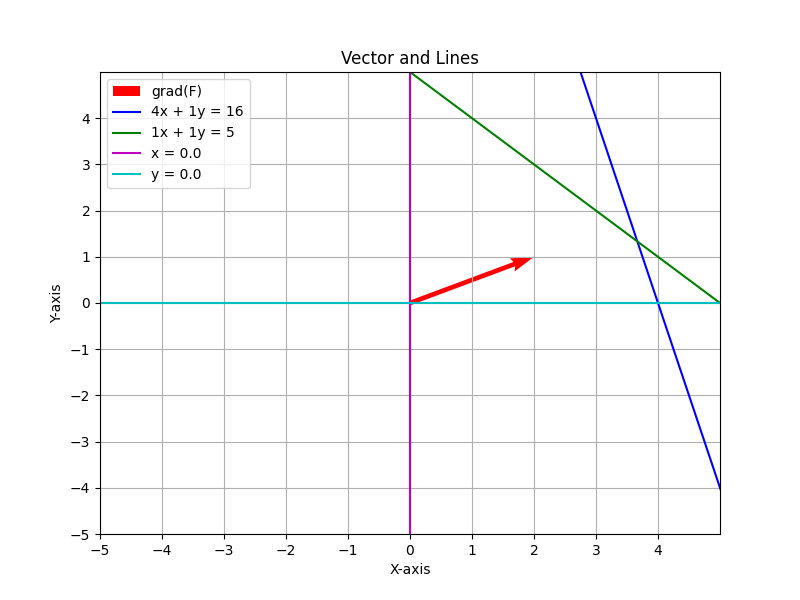
\includegraphics[width=0.7\textwidth]{1.png}
    \caption{Графическое решение задачи}
\end{figure}

\[
    F_{\text{min}} = F(0, 0) = 0, \quad F_{\text{max}} = F\left(\frac{11}{3}, \frac{4}{3}\right) = \frac{26}{3}
\]

\subsection*{2. Решение задачи симплекс-методом}

\[
    F_{\text{min}} = -(-F)_{\text{max}} = -F'_{\text{max}}
\]
\[
    \begin{cases}
        x_1 + 2x_2 + x_3 = 14   \\
        -4x_1 + 3x_2 + x_4 = 12 \\
        x_1 + x_5 = 6           \\
        x_i \geq 0, i=\overline{1, 5}
    \end{cases}
\]

\begin{table}[H]
    \centering
    \begin{tabular}{c|c|cccc|c|c}
        \toprule
        Basis & C base & x0 & x1 & x2 & x3 & B  & reduced\_cost \\
        \midrule
        A2    & 0      & 4  & 1  & 1  & 0  & 16 & 4             \\
        A3    & 0      & 1  & 1  & 0  & 1  & 5  & 5             \\
        \midrule
              & delta  & 2  & 1  & 0  & 0  & 0  &               \\
              & c      & 2  & 1  & 0  & 0  & 0  &               \\
        \bottomrule
    \end{tabular}
\end{table}

\begin{table}[H]
    \centering
    \begin{tabular}{c|c|cccc|c|c}
        \toprule
        Basis & C base & x0 & x1   & x2    & x3 & B & reduced\_cost \\
        \midrule
        A0    & 2.0    & 1  & 0.25 & 0.25  & 0  & 4 & 16            \\
        A3    & 0      & 0  & 0.75 & -0.25 & 1  & 1 & 1.33333       \\
        \midrule
              & delta  & 0  & 0.5  & -0.5  & 0  & 8 &               \\
              & c      & 2  & 1    & 0     & 0  & 0 &               \\
        \bottomrule
    \end{tabular}
\end{table}

\begin{table}[H]
    \centering
    \begin{tabular}{c|c|cccc|c}
        \toprule
        Basis & C base & x0 & x1 & x2        & x3        & B       \\
        \midrule
        A0    & 2.0    & 1  & 0  & 0.333333  & -0.333333 & 3.66667 \\
        A1    & 1.0    & 0  & 1  & -0.333333 & 1.33333   & 1.33333 \\
        \midrule
              & delta  & 0  & 0  & -0.333333 & -0.666667 & 8.66667 \\
              & c      & 2  & 1  & 0         & 0         & 0       \\
        \bottomrule
    \end{tabular}
\end{table}

\[
    F_{\text{max}} = F\left(\frac{11}{3}, \frac{4}{3}\right) = \frac{26}{3}
\]

\begin{table}[H]
    \centering
    \begin{tabular}{c|c|cccc|c}
        \toprule
        Basis & C base & x0 & x1 & x2 & x3 & B  \\
        \midrule
        A2    & 0      & 4  & 1  & 1  & 0  & 16 \\
        A3    & 0      & 1  & 1  & 0  & 1  & 5  \\
        \midrule
              & delta  & -2 & -1 & 0  & 0  & 0  \\
              & c      & -2 & -1 & 0  & 0  & 0  \\
        \bottomrule
    \end{tabular}
\end{table}

\[
    F_{\text{min}} = F(0, 0) = 0
\]

\subsection*{3. Решение задачи методом отсечения Гомори}

Добавляем неравенство:
\[
    \frac{2}{3} - \left(\frac{1}{3} \cdot x_2 + \frac{2}{3} \cdot x_3\right) \leq 0
\]

\subsubsection*{3.1 Геометрическим методом}

\begin{figure}[H]
    \centering
    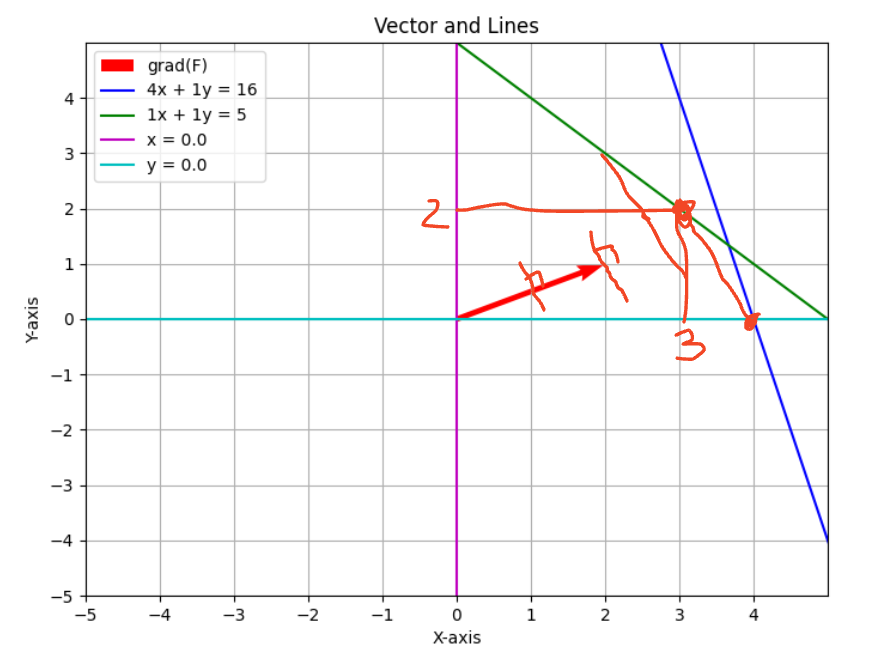
\includegraphics[width=0.7\textwidth]{2.png}
    \caption{Графическое решение задачи с отсечением Гомори}
\end{figure}

\[
    F_{\text{max}} = F(3, 2) = F(4, 0) = 8
\]

\subsubsection*{3.2 Симплекс-методом}

\begin{table}[H]
    \centering
    \begin{tabular}{c|c|cccccc}
        \toprule
        Базис & B     & x1 & x2 & x3   & x4   & x5 \\
        \midrule
        x1    & 11/3  & 1  & 0  & 1/3  & -1/3 & 0  \\
        x2    & 4/3   & 0  & 1  & -1/3 & 4/3  & 0  \\
        x5    & -2/3  & 0  & 0  & -1/3 & -2/3 & 1  \\
        F(X0) & -26/3 & 0  & 0  & -1/3 & -2/3 & 0  \\
        \bottomrule
    \end{tabular}
\end{table}
\[
    \theta_3=-1/3 : (-1/3)=1
    \theta_4=-2/3 : (-2/3)=1
\]

\begin{table}[H]
    \centering
    \begin{tabular}{c|c|cccccc}
        \toprule
        Базис & B  & x1 & x2 & x3  & x4 & x5   \\
        \midrule
        x1    & 4  & 1  & 0  & 1/2 & 0  & -1/2 \\
        x2    & 0  & 0  & 1  & -1  & 0  & 2    \\
        x4    & 1  & 0  & 0  & 1/2 & 1  & -3/2 \\
        F(X0) & -8 & 0  & 0  & 0   & 0  & -1   \\
        \bottomrule
    \end{tabular}
\end{table}

Получили, что \(x_1 = 4\), \(x_2 = 0\), \(F(x_1, x_2) = 8\).

\end{document}